\chapter{Artifact Detection and Localization}

The artifact detection and localization pipeline is responsible for converting the sensor data from the various payloads (Mk. 0, Mk. 1, drone), into a list of artifacts to send to the base station and ultimately report to DARPA. The pipeline was developed to meet a set of requirements, which were derived from the competition rules and our team's concept of operations:

\begin{enumerate}
	\item Reported coordinate of artifact must be within 5m (Euclidean distance) of DARPA-surveyed coordinate
	\item Pipeline must run on-board, either on the Xavier (Mk. 0, Mk. 1), or on part of the NUC (drone)
	\item Artifacts must be transmitted to base station over a lossy wireless link
	\item Pipeline should be capable of detecting all 5 types of artifacts (as shown in Figure \ref{tunnel artifacts})
	\item All artifacts which the robots pass by should be detected
	\item Pipeline should be identical or nearly identical on all payloads
	\item Artifacts should be detected and reported to human supervisor in real-time
\end{enumerate}

Additionally, the following assumptions were made to constrain the scope of the pipeline and guide parameter tuning wherever necessary:

% TODO(vasua): Turn this (and above) into a table
\begin{enumerate}
	\item State estimation system on all payloads would be LOAM
	\item Artifact detection and localization pipeline could not direct robots' exploration
	\item Artifacts are reported in robots' own frames and transformed to a single world frame at base station
	\item Robots will move at approximately 2 m/s
	\item A human supervisor would be available to verify artifact reports, and thus false positives are acceptable
\end{enumerate}

An overview of the complete pipeline is given in Figure \ref{software_overview}. This pipeline runs identically on all 3 payloads with only minor configuration changes (e.g. sensor serial numbers), and sensor omissions where necessary (e.g. drone payload does not contain a thermal camera). All robots report artifacts to the GUI independently, and no information is shared between pipelines running on individual payloads.

\begin{figure}	
	\centering
	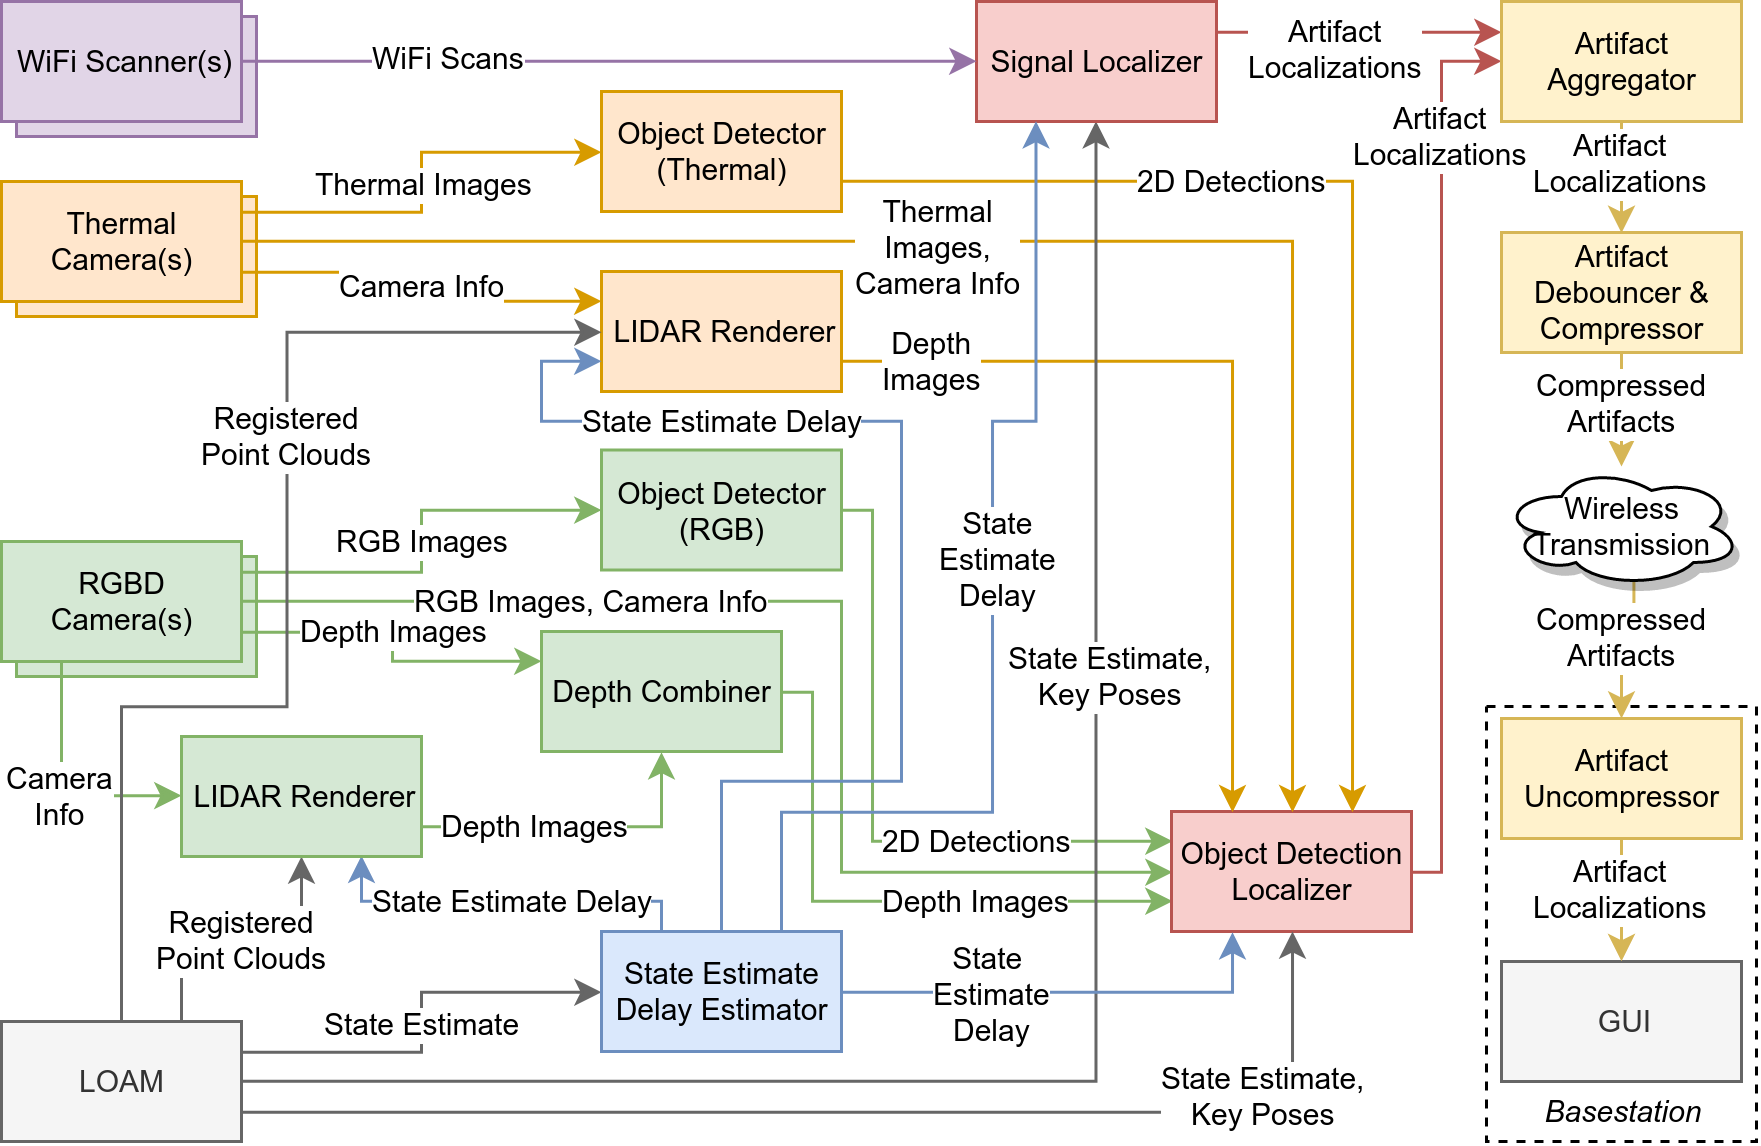
\includegraphics[width=\textwidth]{software_overview.png}
	\caption{Artifact detection and localization software diagram}
	\label{software_overview}
\end{figure}

% TODO(vasua): A better figure for what is inside an artifact localization?
The pipeline consists of 2 major modules - the Signal Localizer and the Object Detection Localizer. Each module takes in various sensor data and produces artifact localizations, which are 3D coordinates in the robot's map frame that are believed to correspond to a desired artifact. These artifact localizations may contain additional evidence to be displayed to the human supervisor, such as images or point clouds of the artifact and surrounding environment. Artifact localizations from both modules are combined inside the Artifact Aggregator and then transmitted to the base station to be displayed on the GUI. The human supervisor inspects artifacts displayed on the GUI and reports valid ones to DARPA.

\section{LOAM Overview}

One of the assumptions made during the initial design phases of the software pipeline was that LOAM would be the state estimation system used on all of our payloads. This simplified the development of the artifact detection and localization pipeline as we only needed to develop and test against a single state estimation system. The relevant interface details of LOAM (in the form of ROS frames and topics) are given below:

\begin{description}
	\item[/sensor] This is the robot's local frame, and is coincident with the Velodyne LIDAR's frame.
	\item[/sensor\_init] The fixed frame used as the base for LOAM's odometry.
	\item[/map] The world frame, which is initially coincident with sensor\_init but can change after loop closures.
	\item[/key\_pose\_to\_map] LOAM creates a series of key poses as the robot traverses the environment. These key poses are generated approximately every 2 meters of the robot's path. Each key pose is given a unique ID, starting from 0. The key pose is published relative to the /map frame.
	\item[/key\_pose\_path] When LOAM detects a loop closure, it corrects the key poses and publishes a new list of key pose IDs and poses.
	\item[/velodyne\_cloud\_registered] The laser scan from the Velodyne LIDAR is aligned to previous scans and published on this topic at 5 Hz. Contrary to key poses, registered scans are published on this topic even when the robot is stationary. The scans are registered in the /sensor\_init frame and accumulate drift over time, but are locally smooth.
	\item[/integrated\_to\_map] The 6DOF pose of the /sensor frame is published on this topic at 200 Hz. The pose is corrected by loop closures and thus does not accumulate significant drift, but may be discontinuous locally.
\end{description}

\section{Object Detector (RGB)}

TODO

\section{Object Detector (Thermal)}

TODO

\section{LIDAR Renderer}

The LIDAR renderer uses camera information (intrinsics and extrinsics) to render depth images. The depth information comes from the registered point clouds from LOAM. For RGB images, the LIDAR renderer provides an alternative source for depth information as depth images are already produced by the RealSense cameras. However, the LIDAR renderer serves as the only source of depth information for the thermal cameras, as they do not otherwise have associated depth information.

\subsection{Implementation}

Two implementations of the LIDAR renderer were created - a reference implementation which ran on CPU, and an optimized one which ran on a GPU using CUDA. The optimized implementation is used on both Mk. 0 and Mk. 1 and runs on the Xavier, where it renders depth images for either 5 or 6 image streams (4x RGB and 1 or 2x thermal). The reference implementation was used to validate the GPU implementation for correctness. The reference implementation also runs on the NUC on the drone payload as it does not have a GPU that supports CUDA. The slower performance of the reference implementation is acceptable as renders only need to be produced for a single RGB stream. Both implementations share the same overall algorithm, comprising two separate methods:

\begin{description}
	\item[Cloud aggregation] The renderer aggregates the registered point clouds from LOAM. A rolling buffer of these clouds is maintained, whose size is proportional to the time it takes to render an image. 10 clouds are stored in the reference implementation, and 30 clouds are stored in the GPU implementation. The clouds are already transformed into a common frame and form a locally smooth point cloud. Global drift is present, but can be ignored since the rendered depth images only see a small local portion of the map.
	\item[Rendering] For each rendered image, the renderer computes the position of the camera in the same frame as the aggregated point clouds. The renderer then uses the camera intrinsics to construct a pinhole camera model and projects each point through it to obtain a location in image coordinates. This coordinate, as well as pixels around this coordinate (based on a configurable inflation parameter) are updated based on the distance to the point, keeping the closer point. The projected coordinates are inflated (as shown in Figure \ref{lidar_inflate}) to provide a denser output image to ensure that depth values are not lost in any potential future downsampling.
\end{description}

\begin{figure}
	\centering
	\begin{subfigure}{0.3\textwidth}
		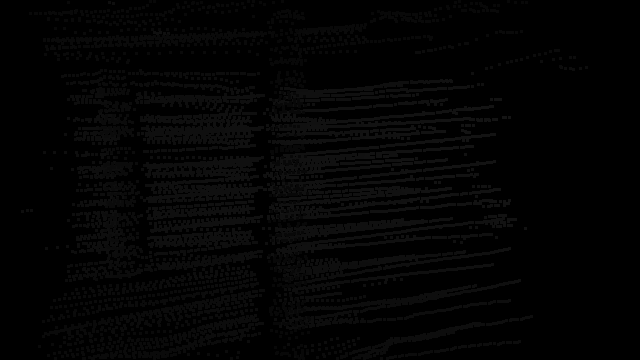
\includegraphics[width=\textwidth]{inflate_1.png}
		\caption{1 pixel inflation}
		\label{inflate_1}
	\end{subfigure}		
	\hfill
	\begin{subfigure}{0.3\textwidth}
		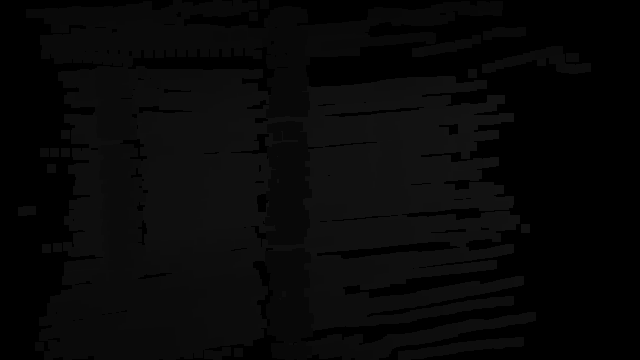
\includegraphics[width=\textwidth]{inflate_4.png}
		\caption{4 pixel inflation}
		\label{inflate_4}		
	\end{subfigure}
	\hfill
	\begin{subfigure}{0.3\textwidth}
		
\includegraphics[width=\textwidth]{inflate_8.png}
		\caption{8 pixel inflation}
		\label{inflate_8}
	\end{subfigure}
	\caption[LIDAR renderer inflation values comparison]{Rendered images of the same scene with different inflation values. An inflation value of 4 was used for all payloads.}
	\label{lidar_inflate}
\end{figure}

\subsection{Results}

A selection of outputs from the LIDAR renderer is given in Figure \ref{lidar_renderer_images}, along with the depth image output from the RealSense camera and the associated RGB image for reference. In the first row, with Mk. 1's camera looking down a long tunnel, the rendered image is significantly sharper and more consistent than that of the RealSense. In the second row, with the left camera looking at a nearby wall, both depth images are similar. In the final row, with a scene from Mk. 1's back camera (which is tilted upwards), the RealSense depth image has significantly fewer holes than the LIDAR's due to the LIDAR's narrow vertical field of view. 

These results show that the output from the LIDAR renderer is either on par with, or better than that from the RealSense cameras, assuming the camera's full field of view is captured by the LIDAR. By fusing both depth images in the Depth Combiner, we can obtain better depth images than either source provides individually.

\begin{figure}
	\centering
	\begin{subfigure}{0.3\textwidth}
		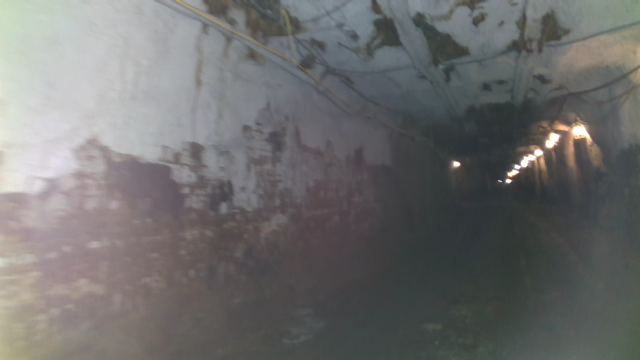
\includegraphics[width=\textwidth]{rs_front_example_2019-10-16-00-51-04_color.png}
		\caption{Mk. 1 Front Color}
		\label{lidar_front_color}
	\end{subfigure}		
	\hfill
	\begin{subfigure}{0.3\textwidth}
		
\includegraphics[width=\textwidth]{rs_front_example_2019-10-16-00-51-04_ref.png}
		\caption{Mk. 1 Front Depth}
		\label{lidar_front_ref}		
	\end{subfigure}
	\hfill
	\begin{subfigure}{0.3\textwidth}
		
\includegraphics[width=\textwidth]{rs_front_example_2019-10-16-00-51-04_render.png}
		\caption{Mk. 1 Front Rendered}
		\label{lidar_front_render}
	\end{subfigure}
	\\
	\begin{subfigure}{0.3\textwidth}
		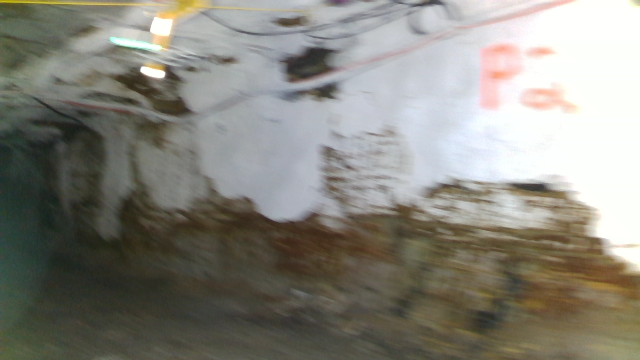
\includegraphics[width=\textwidth]{rs_left_example_2019-10-16-00-51-02_color.png}
		\caption{Mk. 1 Left Color}
		\label{lidar_left_color}
	\end{subfigure}		
	\hfill
	\begin{subfigure}{0.3\textwidth}
		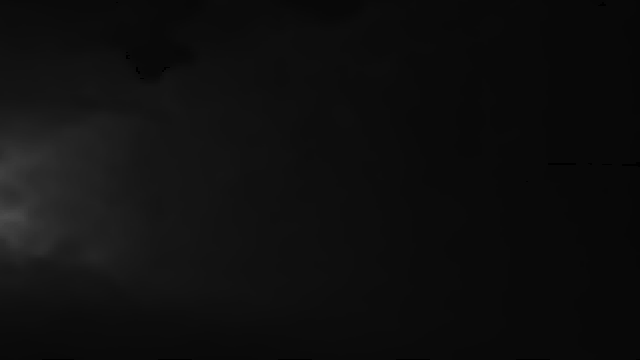
\includegraphics[width=\textwidth]{rs_left_example_2019-10-16-00-51-02_ref.png}
		\caption{Mk. 1 Left Depth}
		\label{lidar_left_ref}		
	\end{subfigure}
	\hfill
	\begin{subfigure}{0.3\textwidth}
		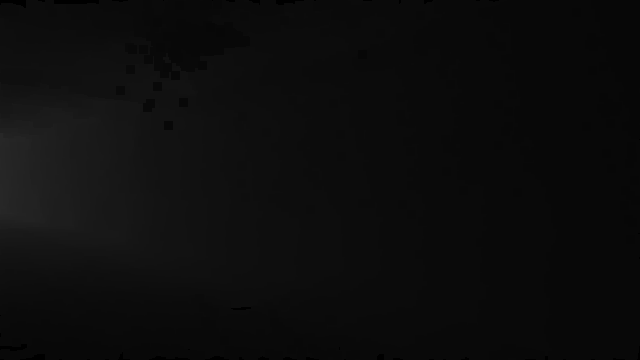
\includegraphics[width=\textwidth]{rs_left_example_2019-10-16-00-51-02_render.png}
		\caption{Mk. 1 Left Rendered}
		\label{lidar_left_render}
	\end{subfigure}
	\\
	\begin{subfigure}{0.3\textwidth}
		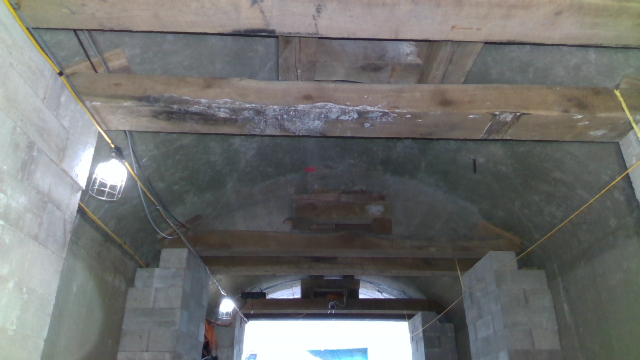
\includegraphics[width=\textwidth]{rs_back_example_2019-10-16-00-33-41_color.png}
		\caption{Mk. 1 Back Color}
		\label{lidar_back_color}
	\end{subfigure}		
	\hfill
	\begin{subfigure}{0.3\textwidth}
		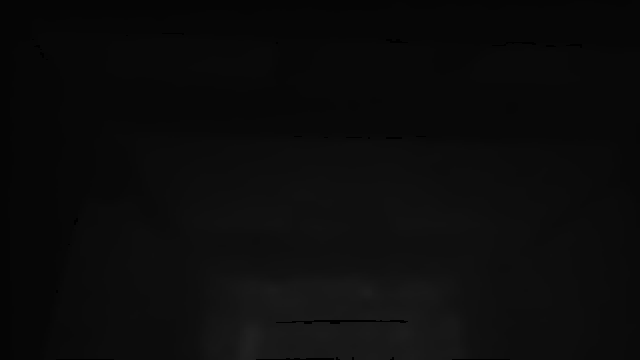
\includegraphics[width=\textwidth]{rs_back_example_2019-10-16-00-33-41_ref.png}
		\caption{Mk. 1 Back Depth}
		\label{lidar_back_ref}		
	\end{subfigure}
	\hfill
	\begin{subfigure}{0.3\textwidth}
		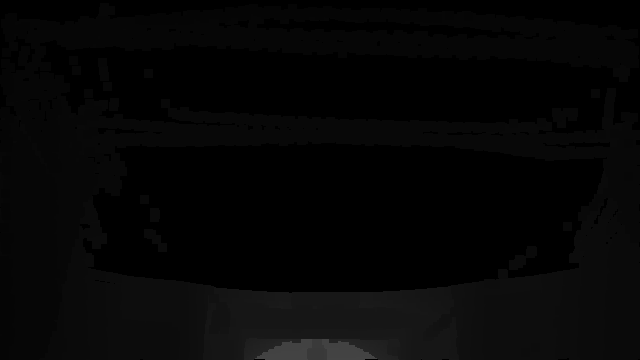
\includegraphics[width=\textwidth]{rs_back_example_2019-10-16-00-33-41_render.png}
		\caption{Mk. 1 Back Rendered}
		\label{lidar_back_render}
	\end{subfigure}		
	\caption[LIDAR renderer depth image comparison]{Comparison of depth images generated by the LIDAR renderer to depth images from the RealSense cameras. Color images, captured simultaneously by the RealSense cameras, are provided for reference.}
	\label{lidar_renderer_images}
\end{figure}

\section{Depth Combiner}

The depth combiner fuses depth images from the RealSense depth camera and LIDAR renderer into a single depth image to be used in the object detection localizer. The two image streams are aligned, and can thus be fused per-pixel. The following equation was used (shown as C++ code):

\begin{lstlisting}[language=c++]
fused = (realsense > threshold || realsense == 0) ? lidar : realsense;
\end{lstlisting}

This fusion keeps lidar data whenever the reported RealSense data is either not present (\lstinline[language=c++]{realsense = 0}) or exceeds some threshold (\lstinline[language=c++]{realsense > threshold}). The threshold empirically selected to be 2.5m, which is the approximate distance after which we observed significant variance in reported depth values between frames. This fusion allows us to use the high density RealSense depth information whenever it is available and sufficiently accurate (under the 2.5m threshold), and utilize the sparser LIDAR information otherwise. An example output is given in Figure \ref{combined_depth}.

\begin{figure}
	\centering
	\begin{subfigure}{0.3\textwidth}
		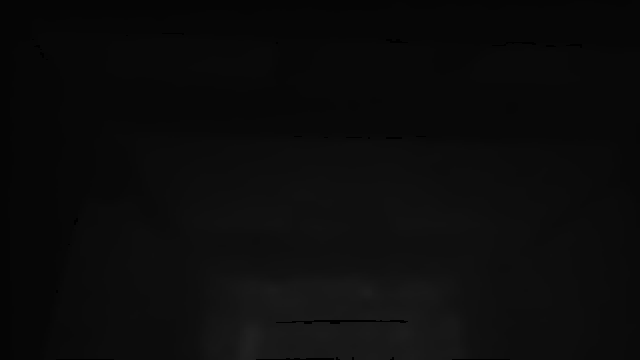
\includegraphics[width=\textwidth]{rs_back_example_2019-10-16-00-33-41_ref.png}
		\caption{Mk. 1 Back Depth}
		\label{combined_depth_realsense}		
	\end{subfigure}
	\hfill
	\begin{subfigure}{0.3\textwidth}
		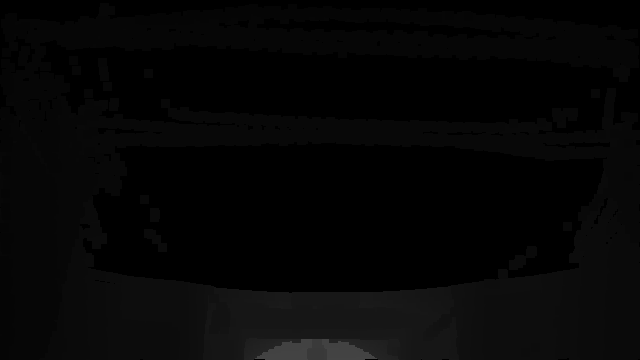
\includegraphics[width=\textwidth]{rs_back_example_2019-10-16-00-33-41_render.png}
		\caption{Mk. 1 Back Rendered}
		\label{combined_depth_lidar}
	\end{subfigure}	
	\hfill
	\begin{subfigure}{0.3\textwidth}
		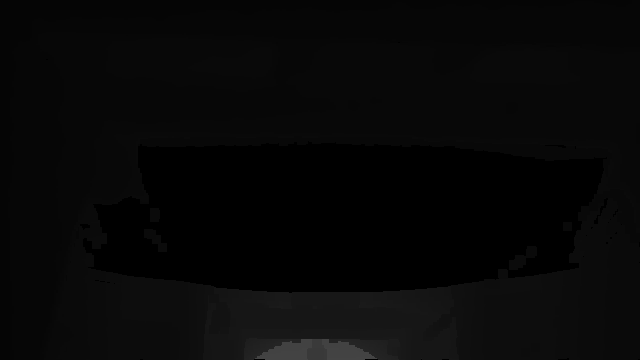
\includegraphics[width=\textwidth]{combined_depth.png}
		\caption{Mk. 1 Back Combined}
		\label{combined_depth_output}
	\end{subfigure}		
	\caption[Depth combiner sample output]{Example of the output from the depth combiner, using the same scene as in \ref{lidar_back_color}.}
	\label{combined_depth}
\end{figure}


\section{Object Detection Localizer}

TODO

\section{WiFi Scanner}

TODO

\section{Signal Localizer}

TODO

\section{State Estimate Delay Estimator}

TODO

\section{Artifact Aggregator}

TODO

\section{Artifact Debouncer \& Compressor}

TODO

\section{Artifact Uncompressor}

TODO

\section{GUI}